\appendix
\renewcommand{\thesection}{APPENDIX \Alph{section}}
\section{ -- Figures} \label{appendix:A}
\topskip0pt
\vspace*{\fill}
\begin{center}
    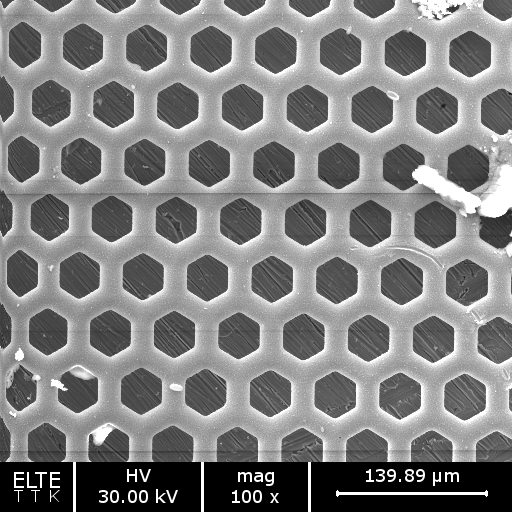
\includegraphics[width=0.8\textwidth]{{img_src/001_a}.png}
    \captionof{figure}{Surface of a microscopic copper lattice with 100x magnitude by detecting secondary electrons.} \label{fig:1}
\end{center}
\begin{center}
    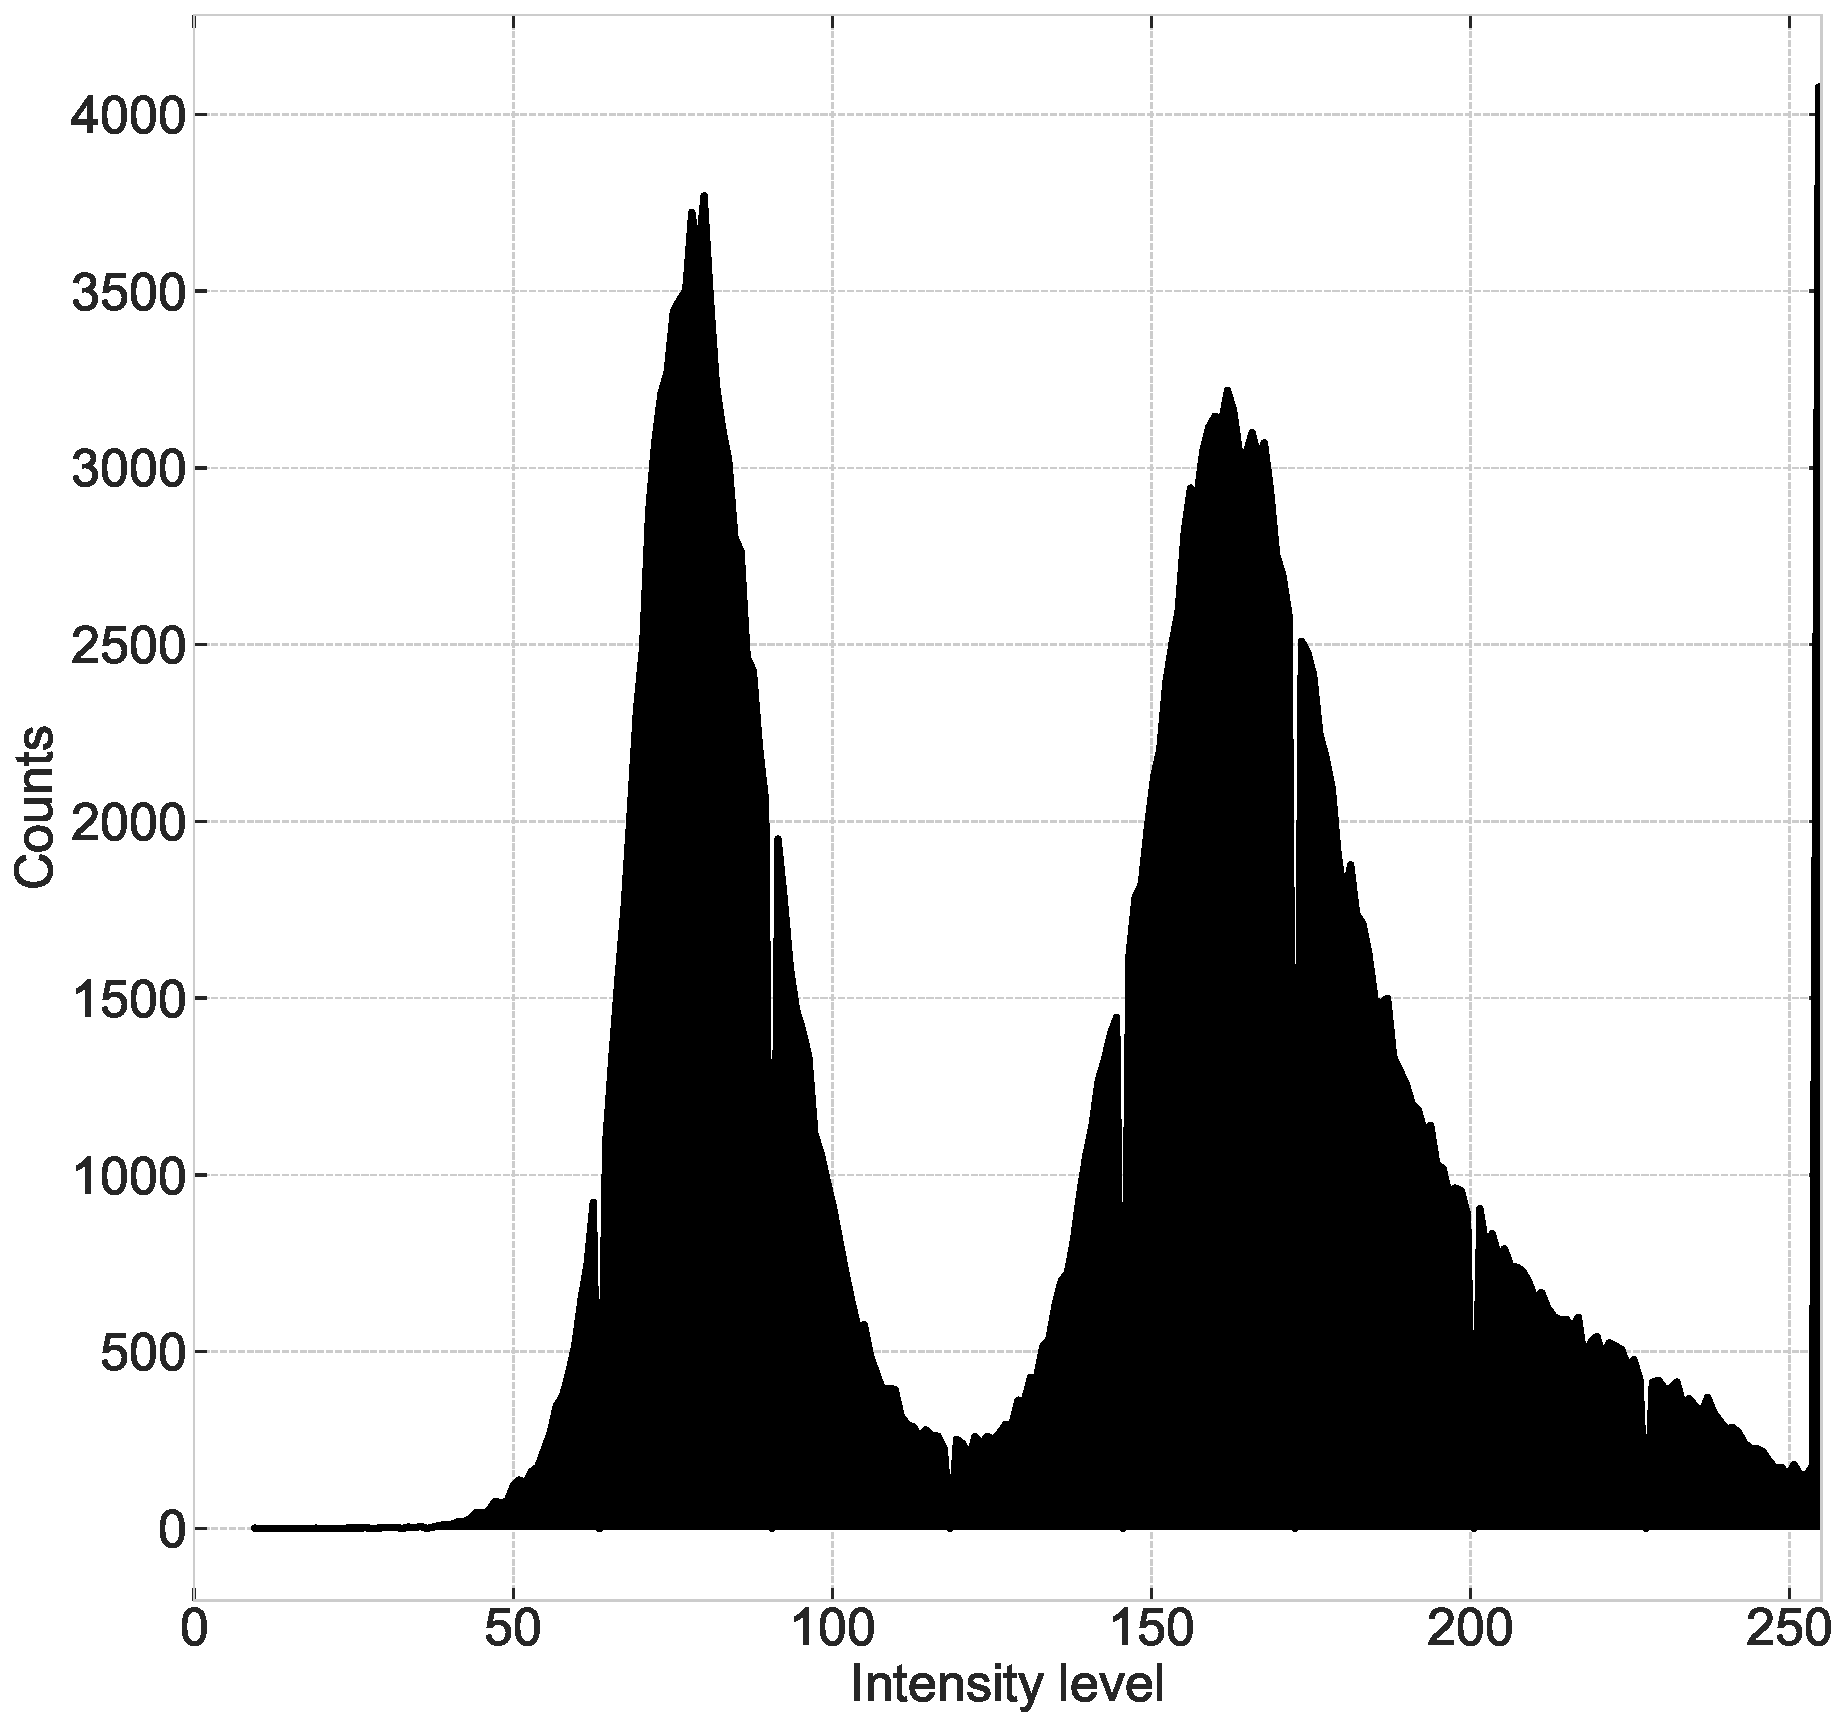
\includegraphics[width=0.8\textwidth]{{img_src/001_a_hist}.pdf}
    \captionof{figure}{Histogram of the image of the microscopic copper lattice with 100x magnitude by detecting secondary electrons.} \label{fig:2}
\end{center}
\vspace*{\fill}
\newpage
\topskip0pt
\vspace*{\fill}
\begin{center}
    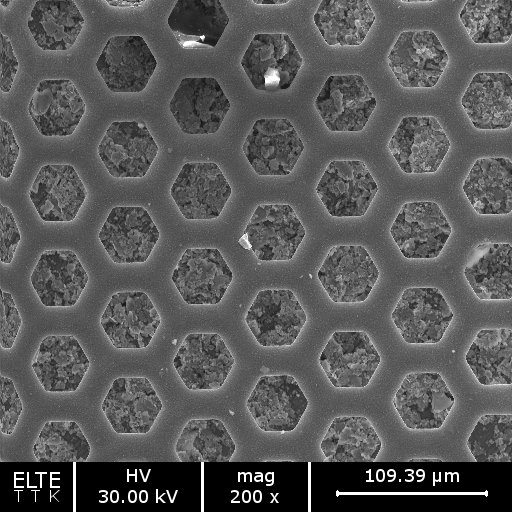
\includegraphics[width=0.8\textwidth]{{img_src/004_a}.png}
    \captionof{figure}{Surface of a microscopic copper lattice with 200x magnitude by detecting secondary electrons.} \label{fig:3}
\end{center}
\begin{center}
    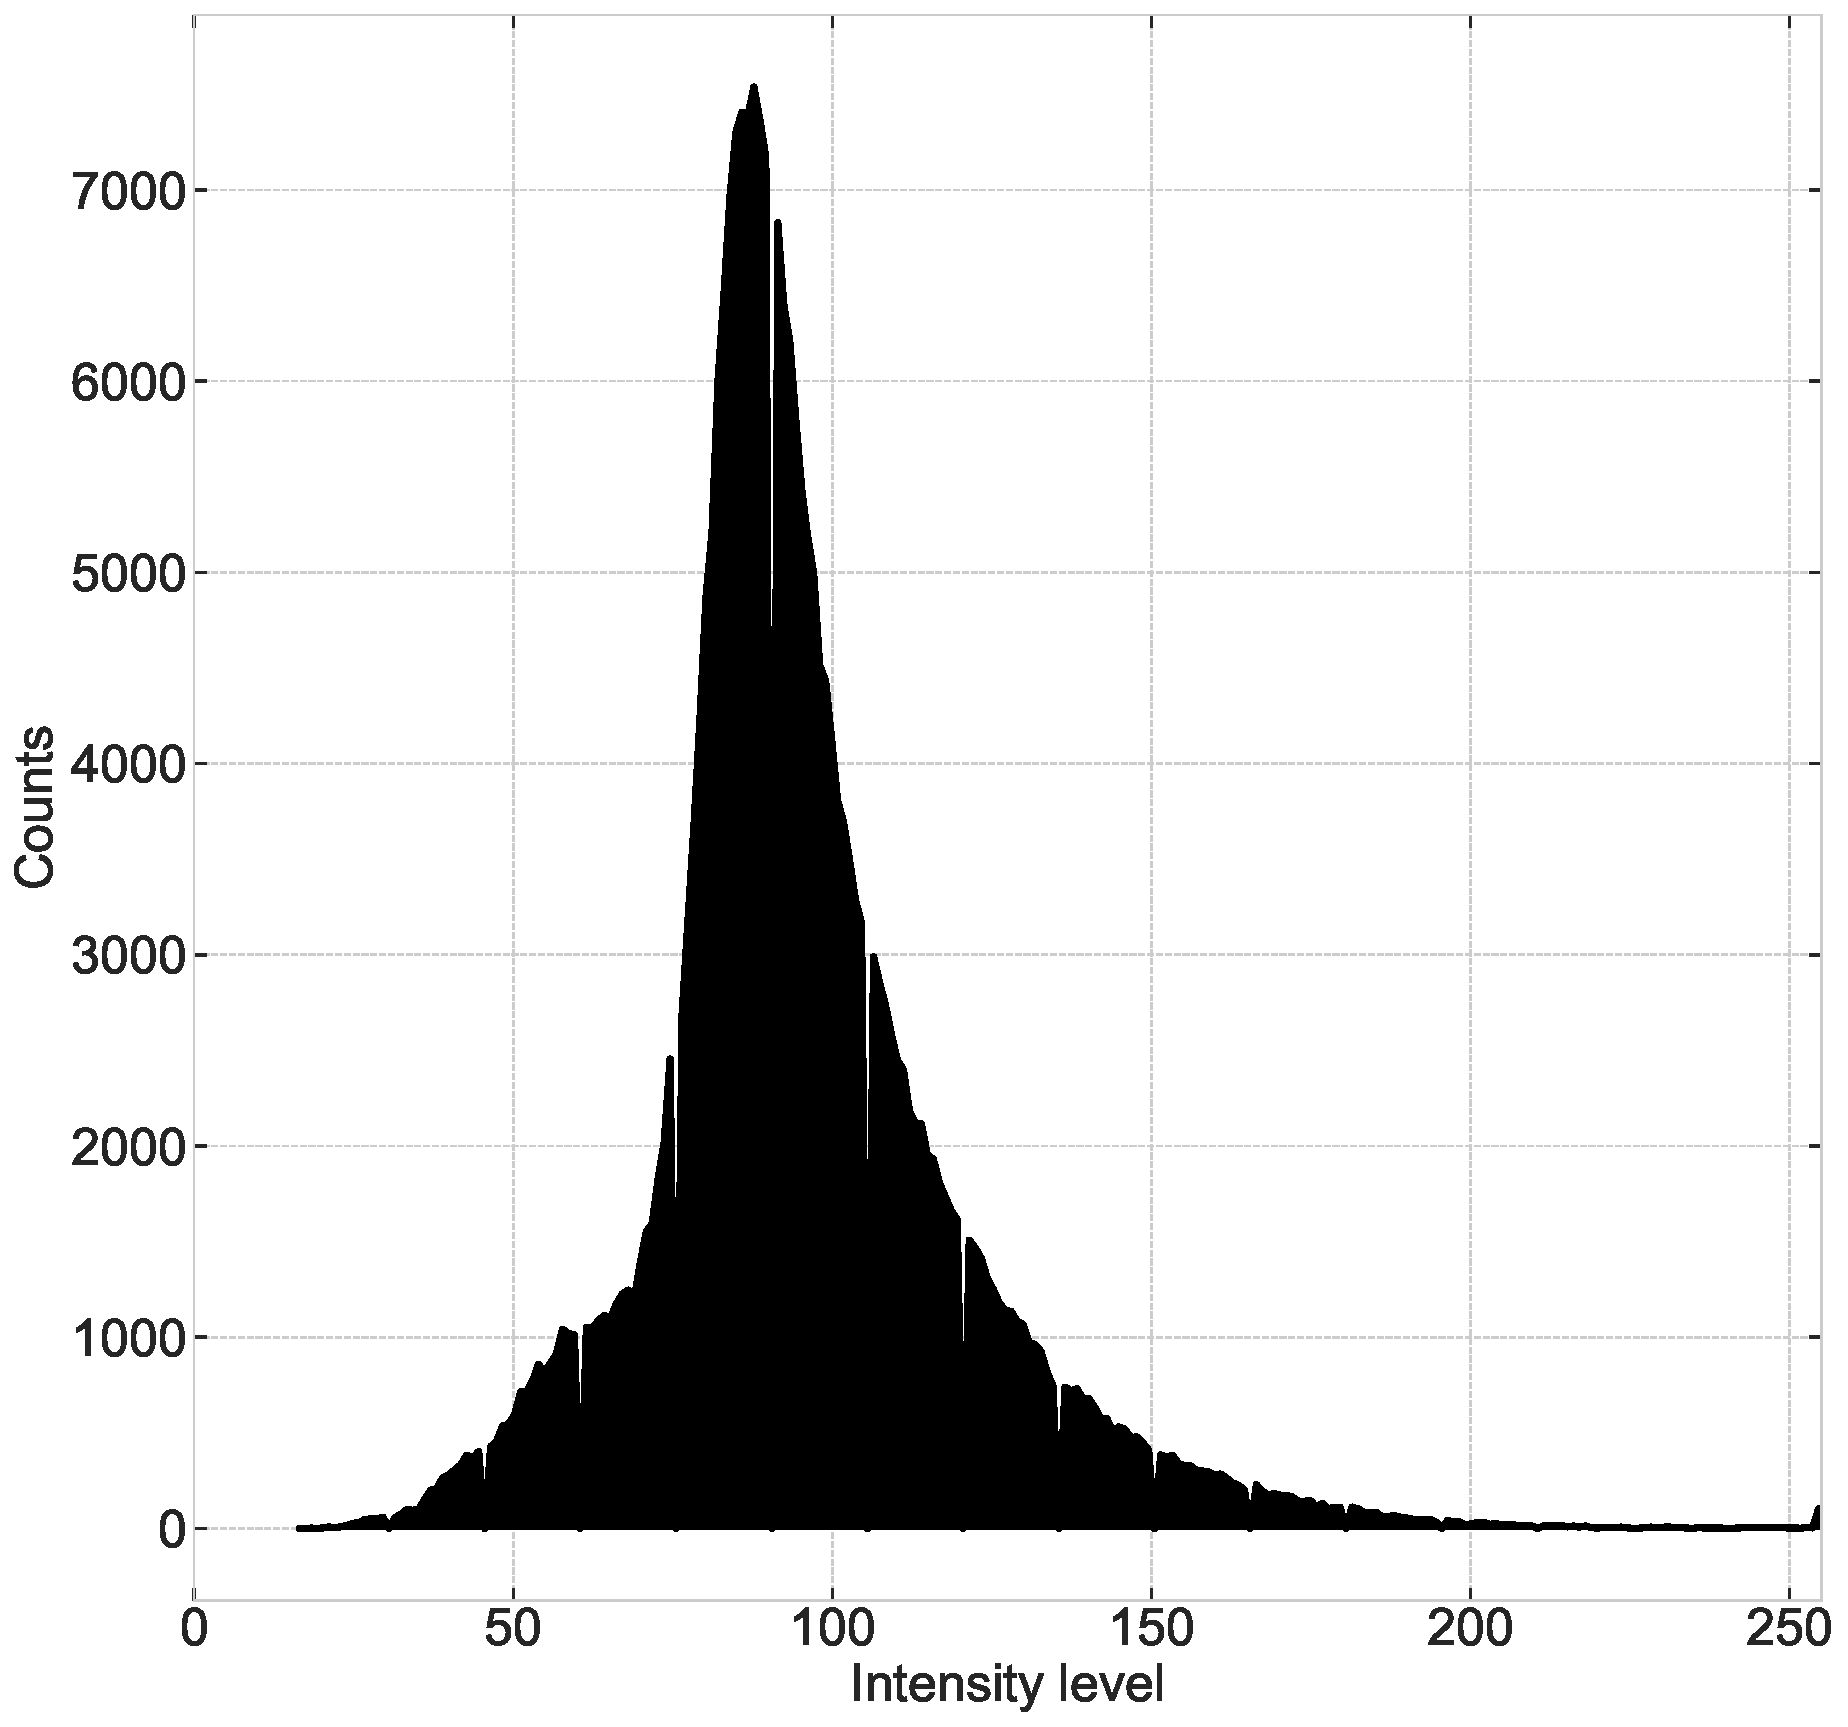
\includegraphics[width=0.8\textwidth]{{img_src/004_a_hist}.pdf}
    \captionof{figure}{Histogram of the image of the microscopic copper lattice with 200x magnitude by detecting secondary electrons.} \label{fig:4}
\end{center}
\vspace*{\fill}
\newpage
\topskip0pt
\vspace*{\fill}
\begin{center}
    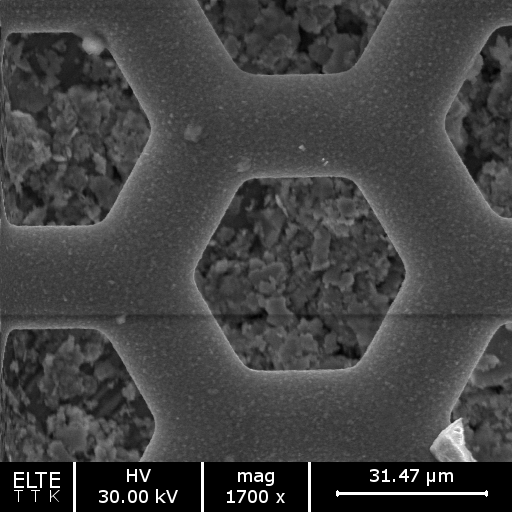
\includegraphics[width=0.8\textwidth]{{img_src/003_a}.png}
    \captionof{figure}{Surface of a microscopic copper lattice with 700x magnitude by detecting secondary electrons.} \label{fig:5}
\end{center}
\begin{center}
    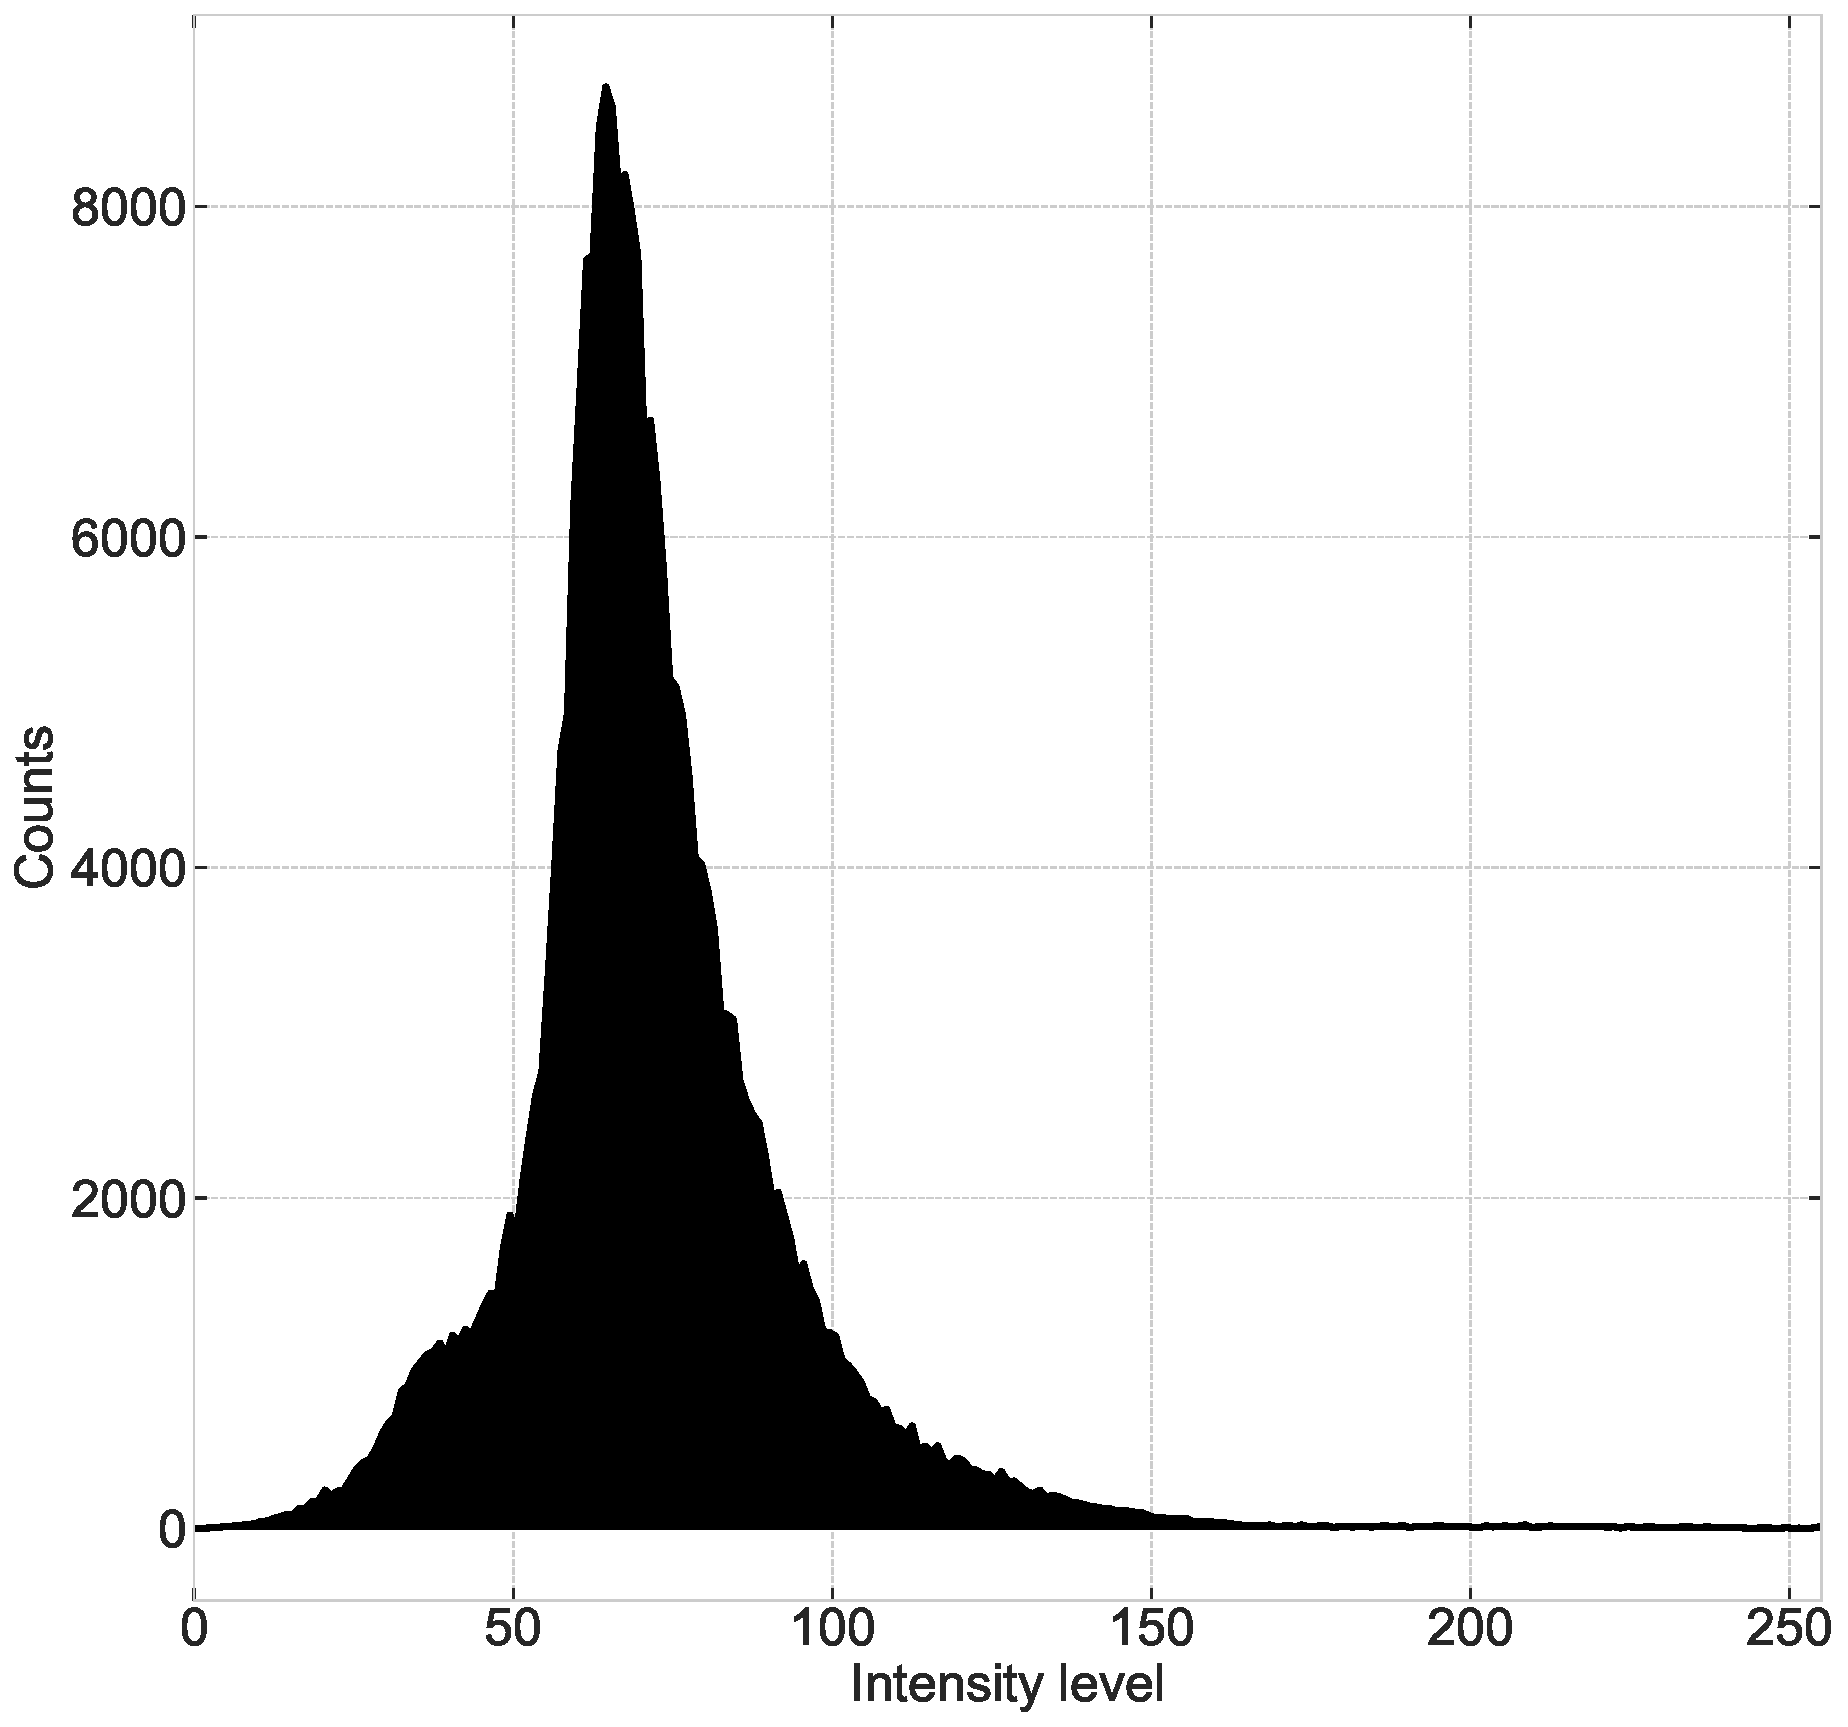
\includegraphics[width=0.8\textwidth]{{img_src/003_a_hist}.pdf}
    \captionof{figure}{Histogram of the image of the microscopic copper lattice with 700x magnitude by detecting secondary electrons.} \label{fig:6}
\end{center}
\vspace*{\fill}
\newpage
\topskip0pt
\vspace*{\fill}
\begin{center}
    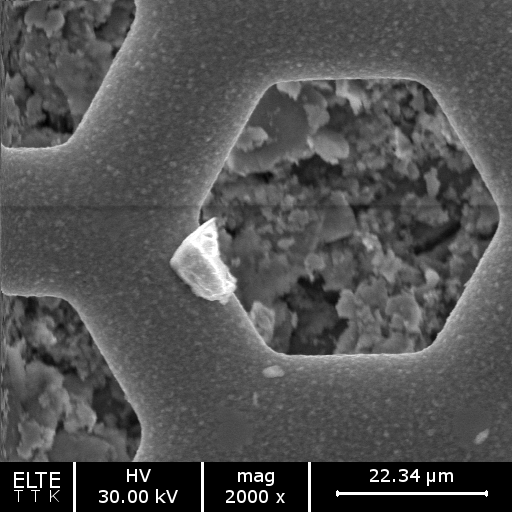
\includegraphics[width=0.8\textwidth]{{img_src/002_a}.png}
    \captionof{figure}{Surface of a microscopic copper lattice with 2000x magnitude by detecting secondary electrons. On the copper grid also some contamination could be seen.} \label{fig:7}
\end{center}
\begin{center}
    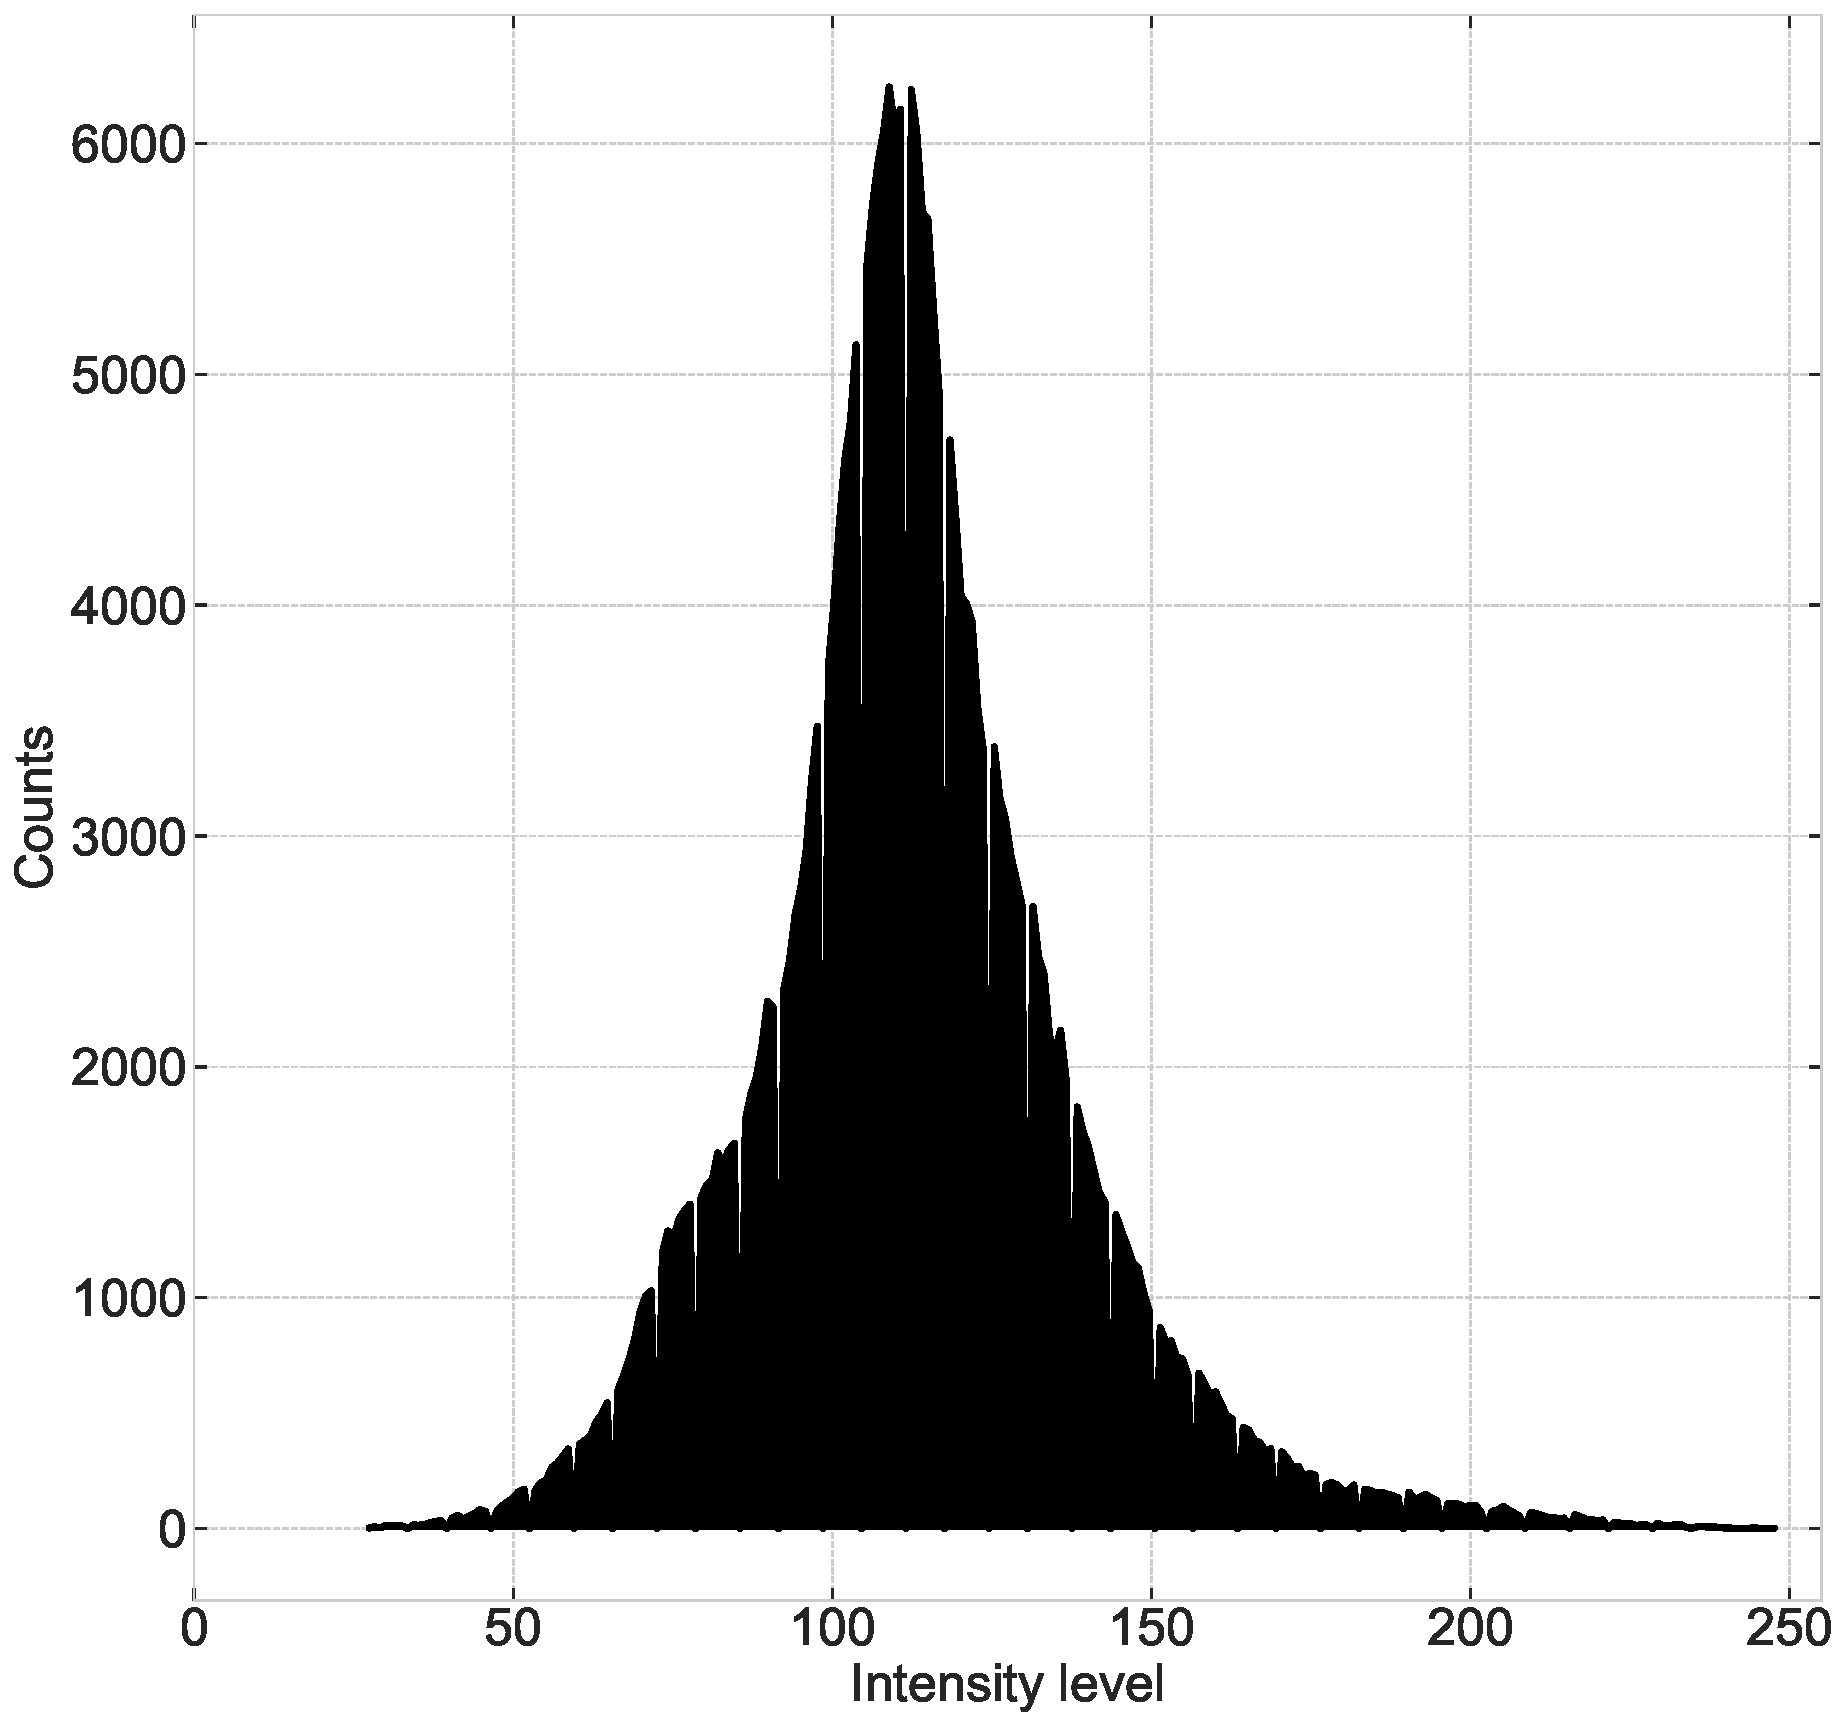
\includegraphics[width=0.8\textwidth]{{img_src/002_a_hist}.pdf}
    \captionof{figure}{Histogram of the image of the microscopic copper lattice with 2000x magnitude by detecting secondary electrons. On the copper grid also some contamination could be seen.} \label{fig:8}
\end{center}
\vspace*{\fill}
\newpage
\topskip0pt
\vspace*{\fill}
\begin{center}
    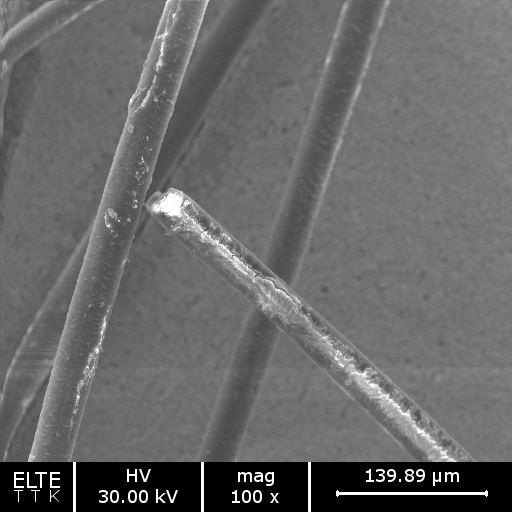
\includegraphics[width=0.8\textwidth]{{img_src/006_a}.png}
    \captionof{figure}{Surface of a human hair with 100x magnitude by detecting secondary electrons.} \label{fig:9}
\end{center}
\begin{center}
    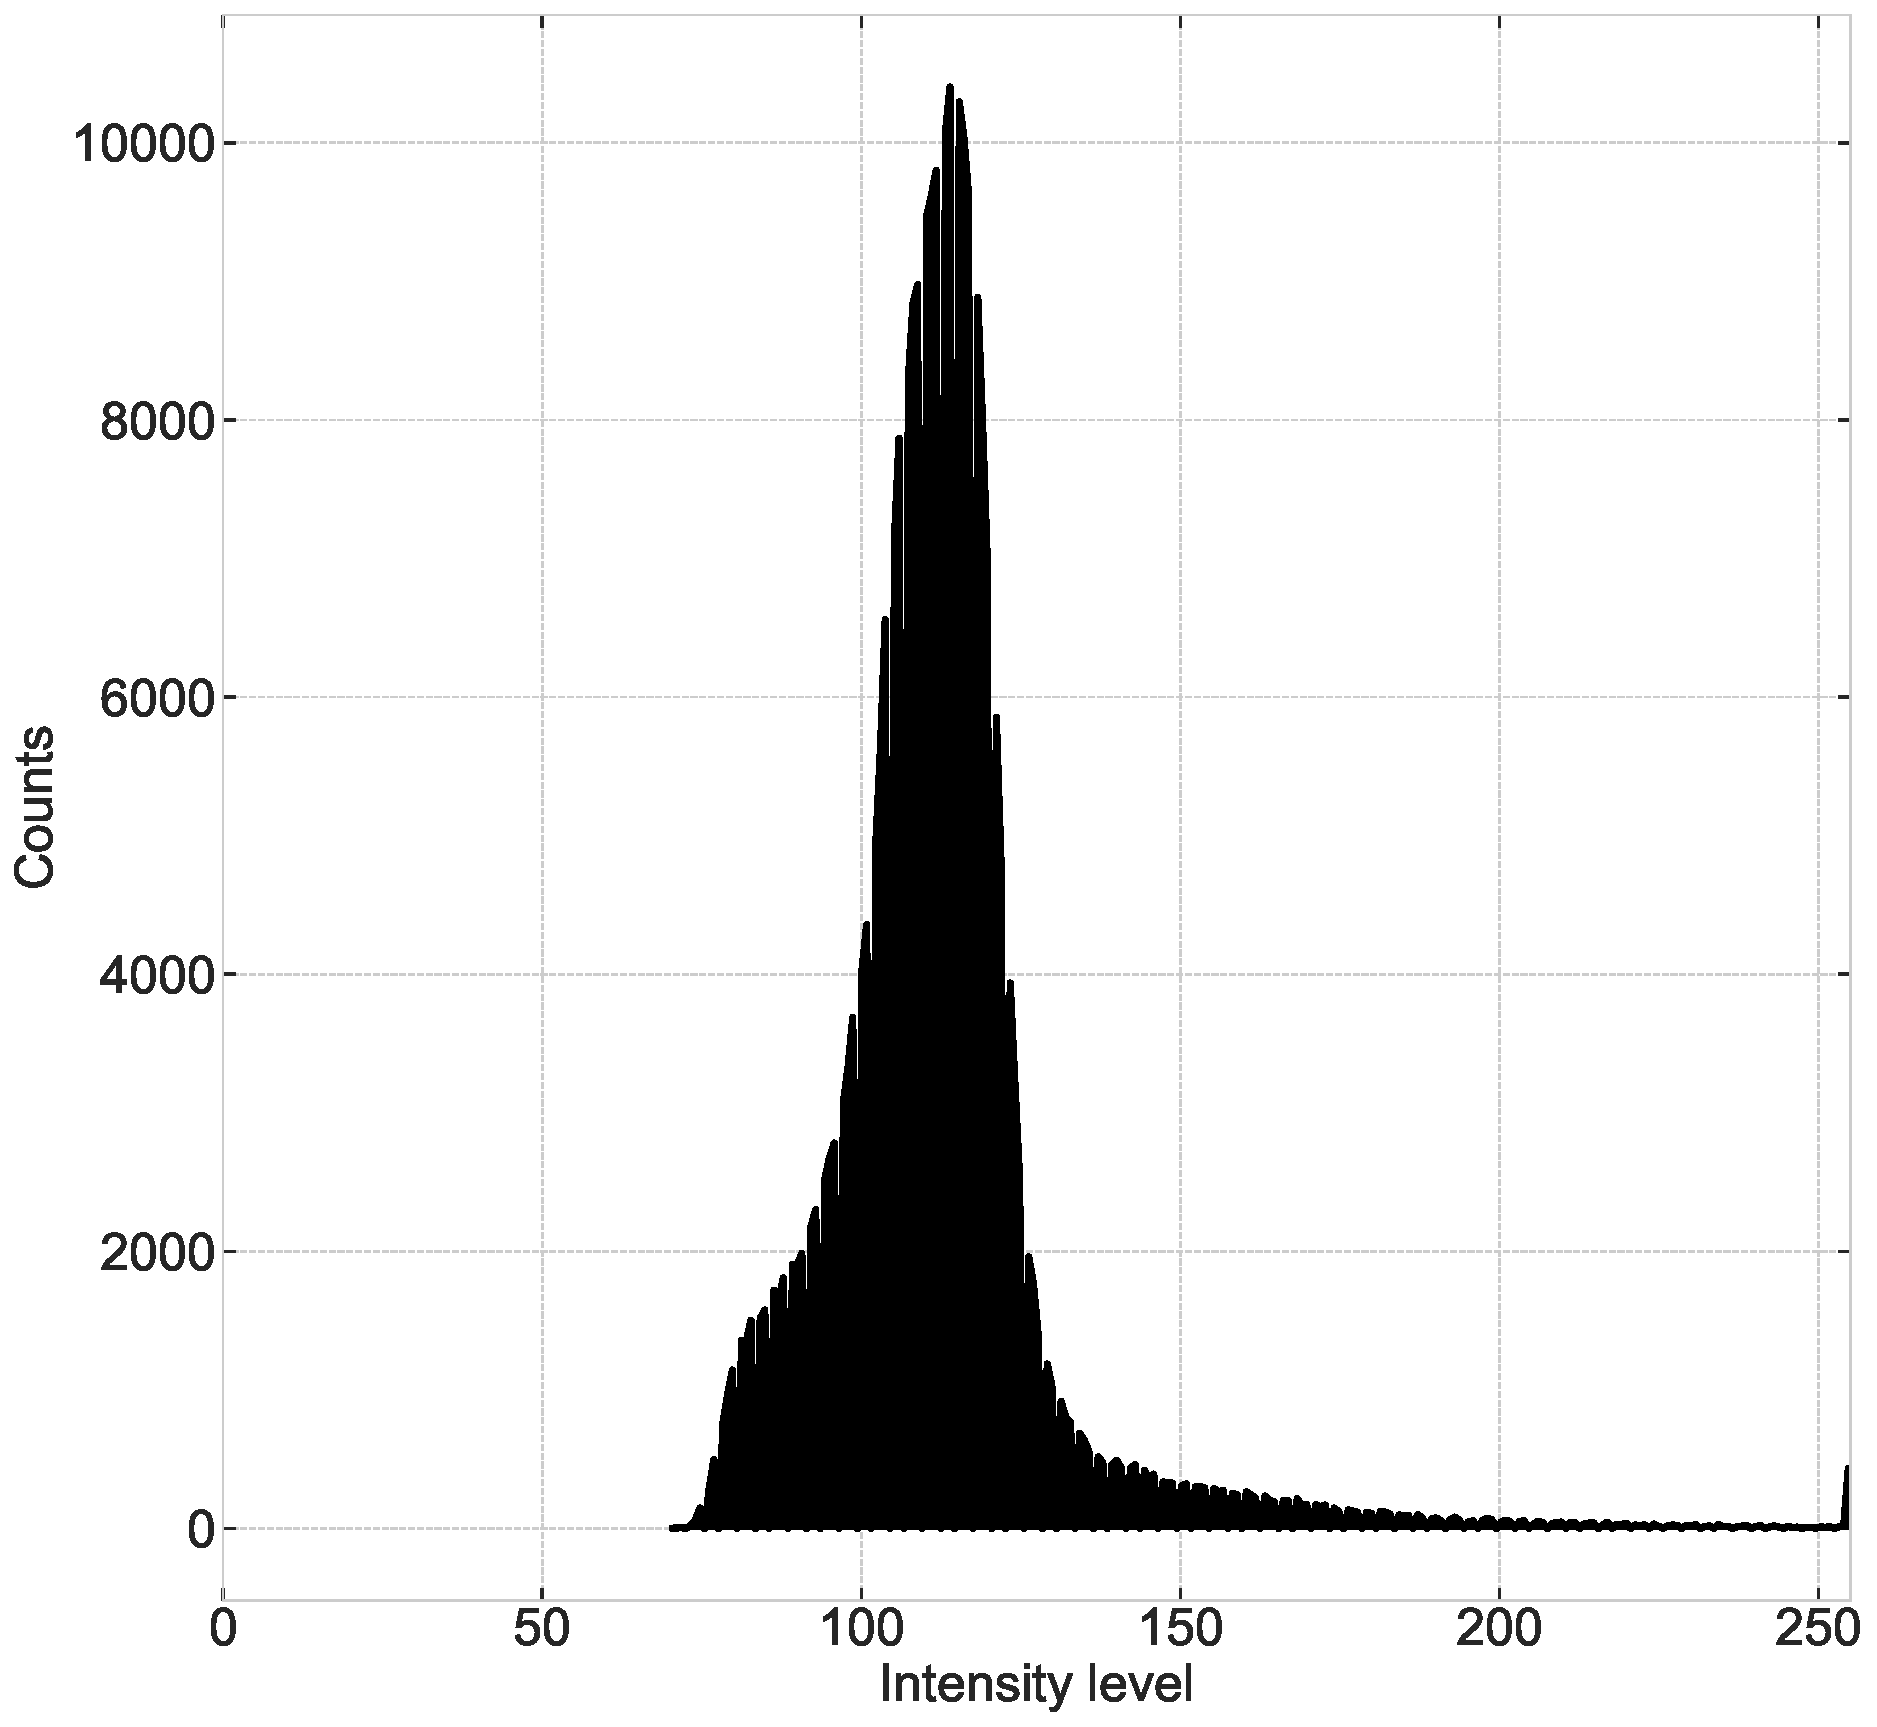
\includegraphics[width=0.8\textwidth]{{img_src/006_a_hist}.pdf}
    \captionof{figure}{Histogram of the image of the human hair with 100x magnitude by detecting secondary electrons.} \label{fig:10}
\end{center}
\vspace*{\fill}
\newpage
\topskip0pt
\vspace*{\fill}
\begin{center}
    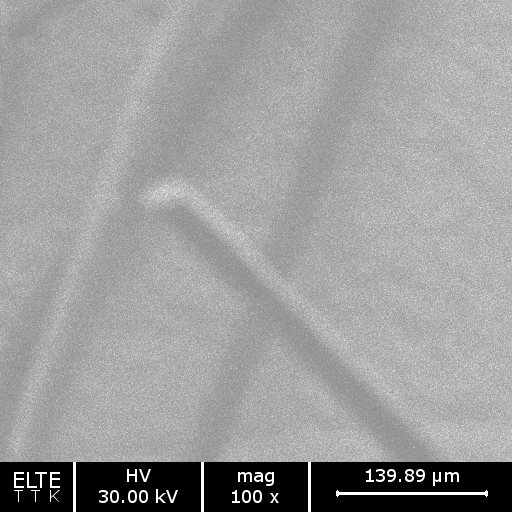
\includegraphics[width=0.8\textwidth]{{img_src/007_a}.png}
    \captionof{figure}{Surface of a human hair with 100x magnitude by detecting backscattered electrons.} \label{fig:11}
\end{center}
\begin{center}
    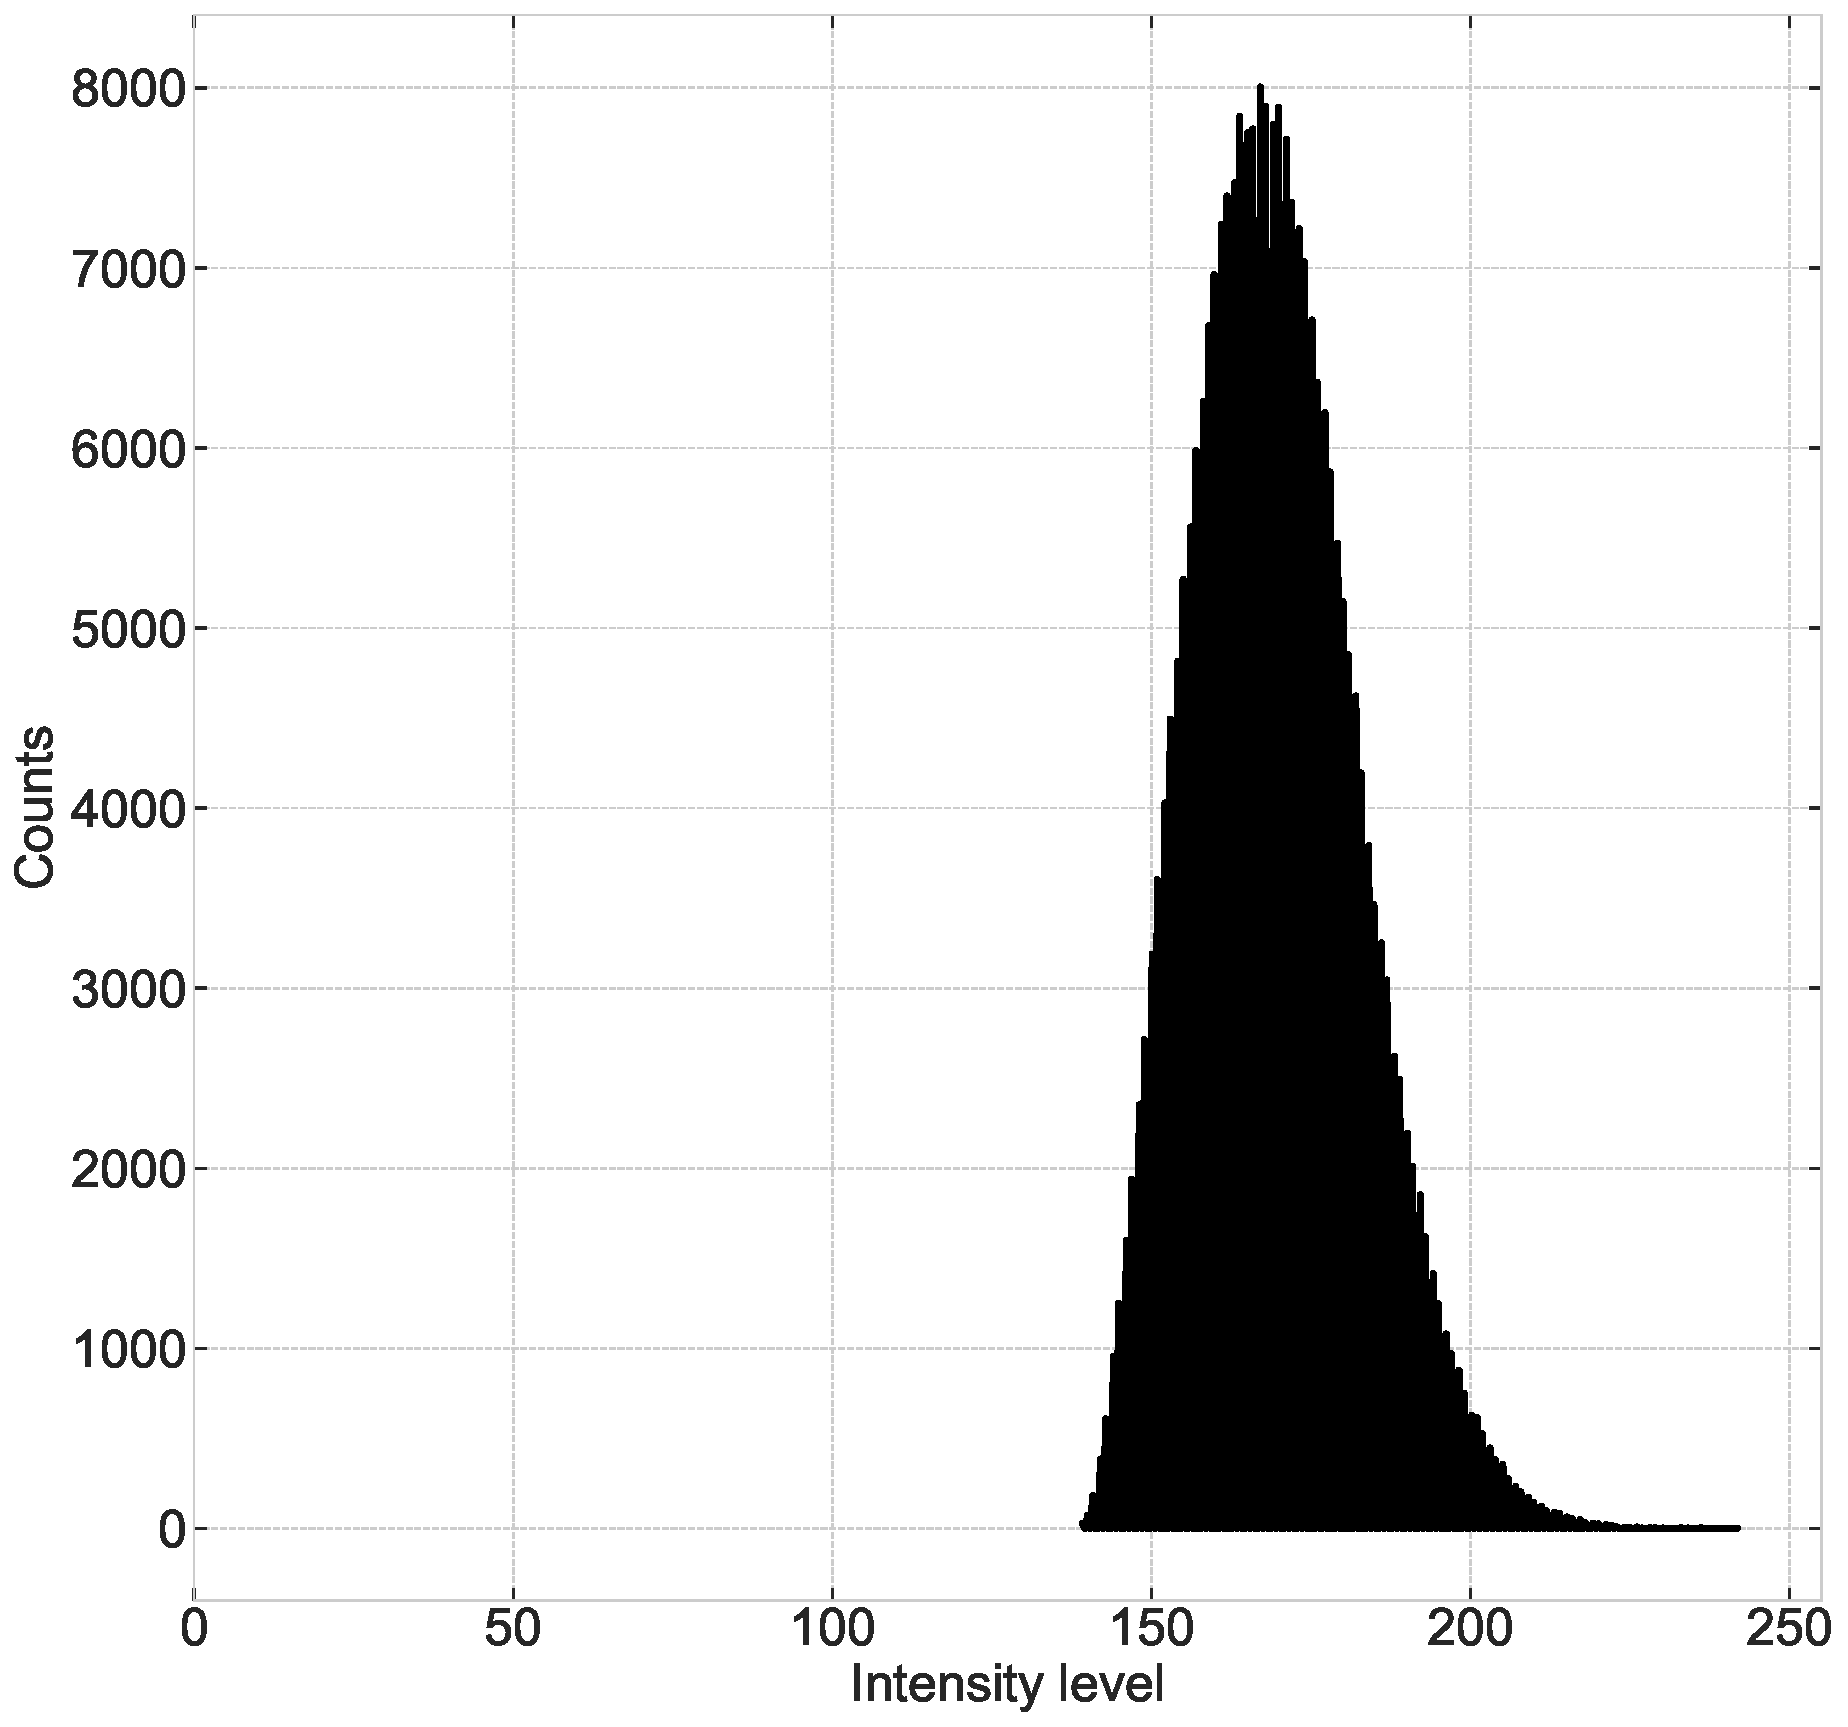
\includegraphics[width=0.8\textwidth]{{img_src/007_a_hist}.pdf}
    \captionof{figure}{Histogram of the image of the human hair with 100x magnitude by detecting backscattered electrons.} \label{fig:12}
\end{center}
\vspace*{\fill}
\newpage
\topskip0pt
\vspace*{\fill}
\begin{center}
    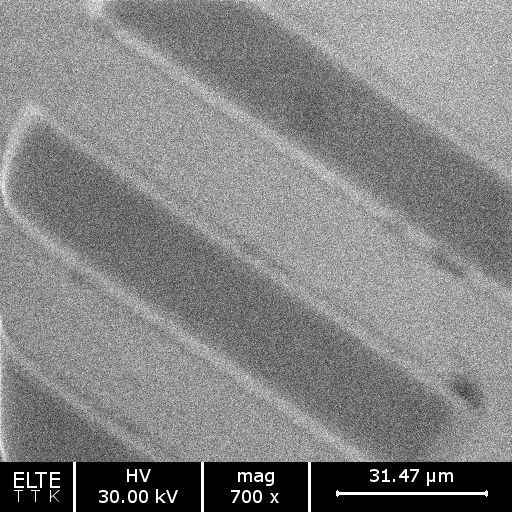
\includegraphics[width=0.8\textwidth]{{img_src/008_a}.png}
    \captionof{figure}{Surface of a microchip with 700x magnitude by detecting secondary electrons.} \label{fig:13}
\end{center}
\begin{center}
    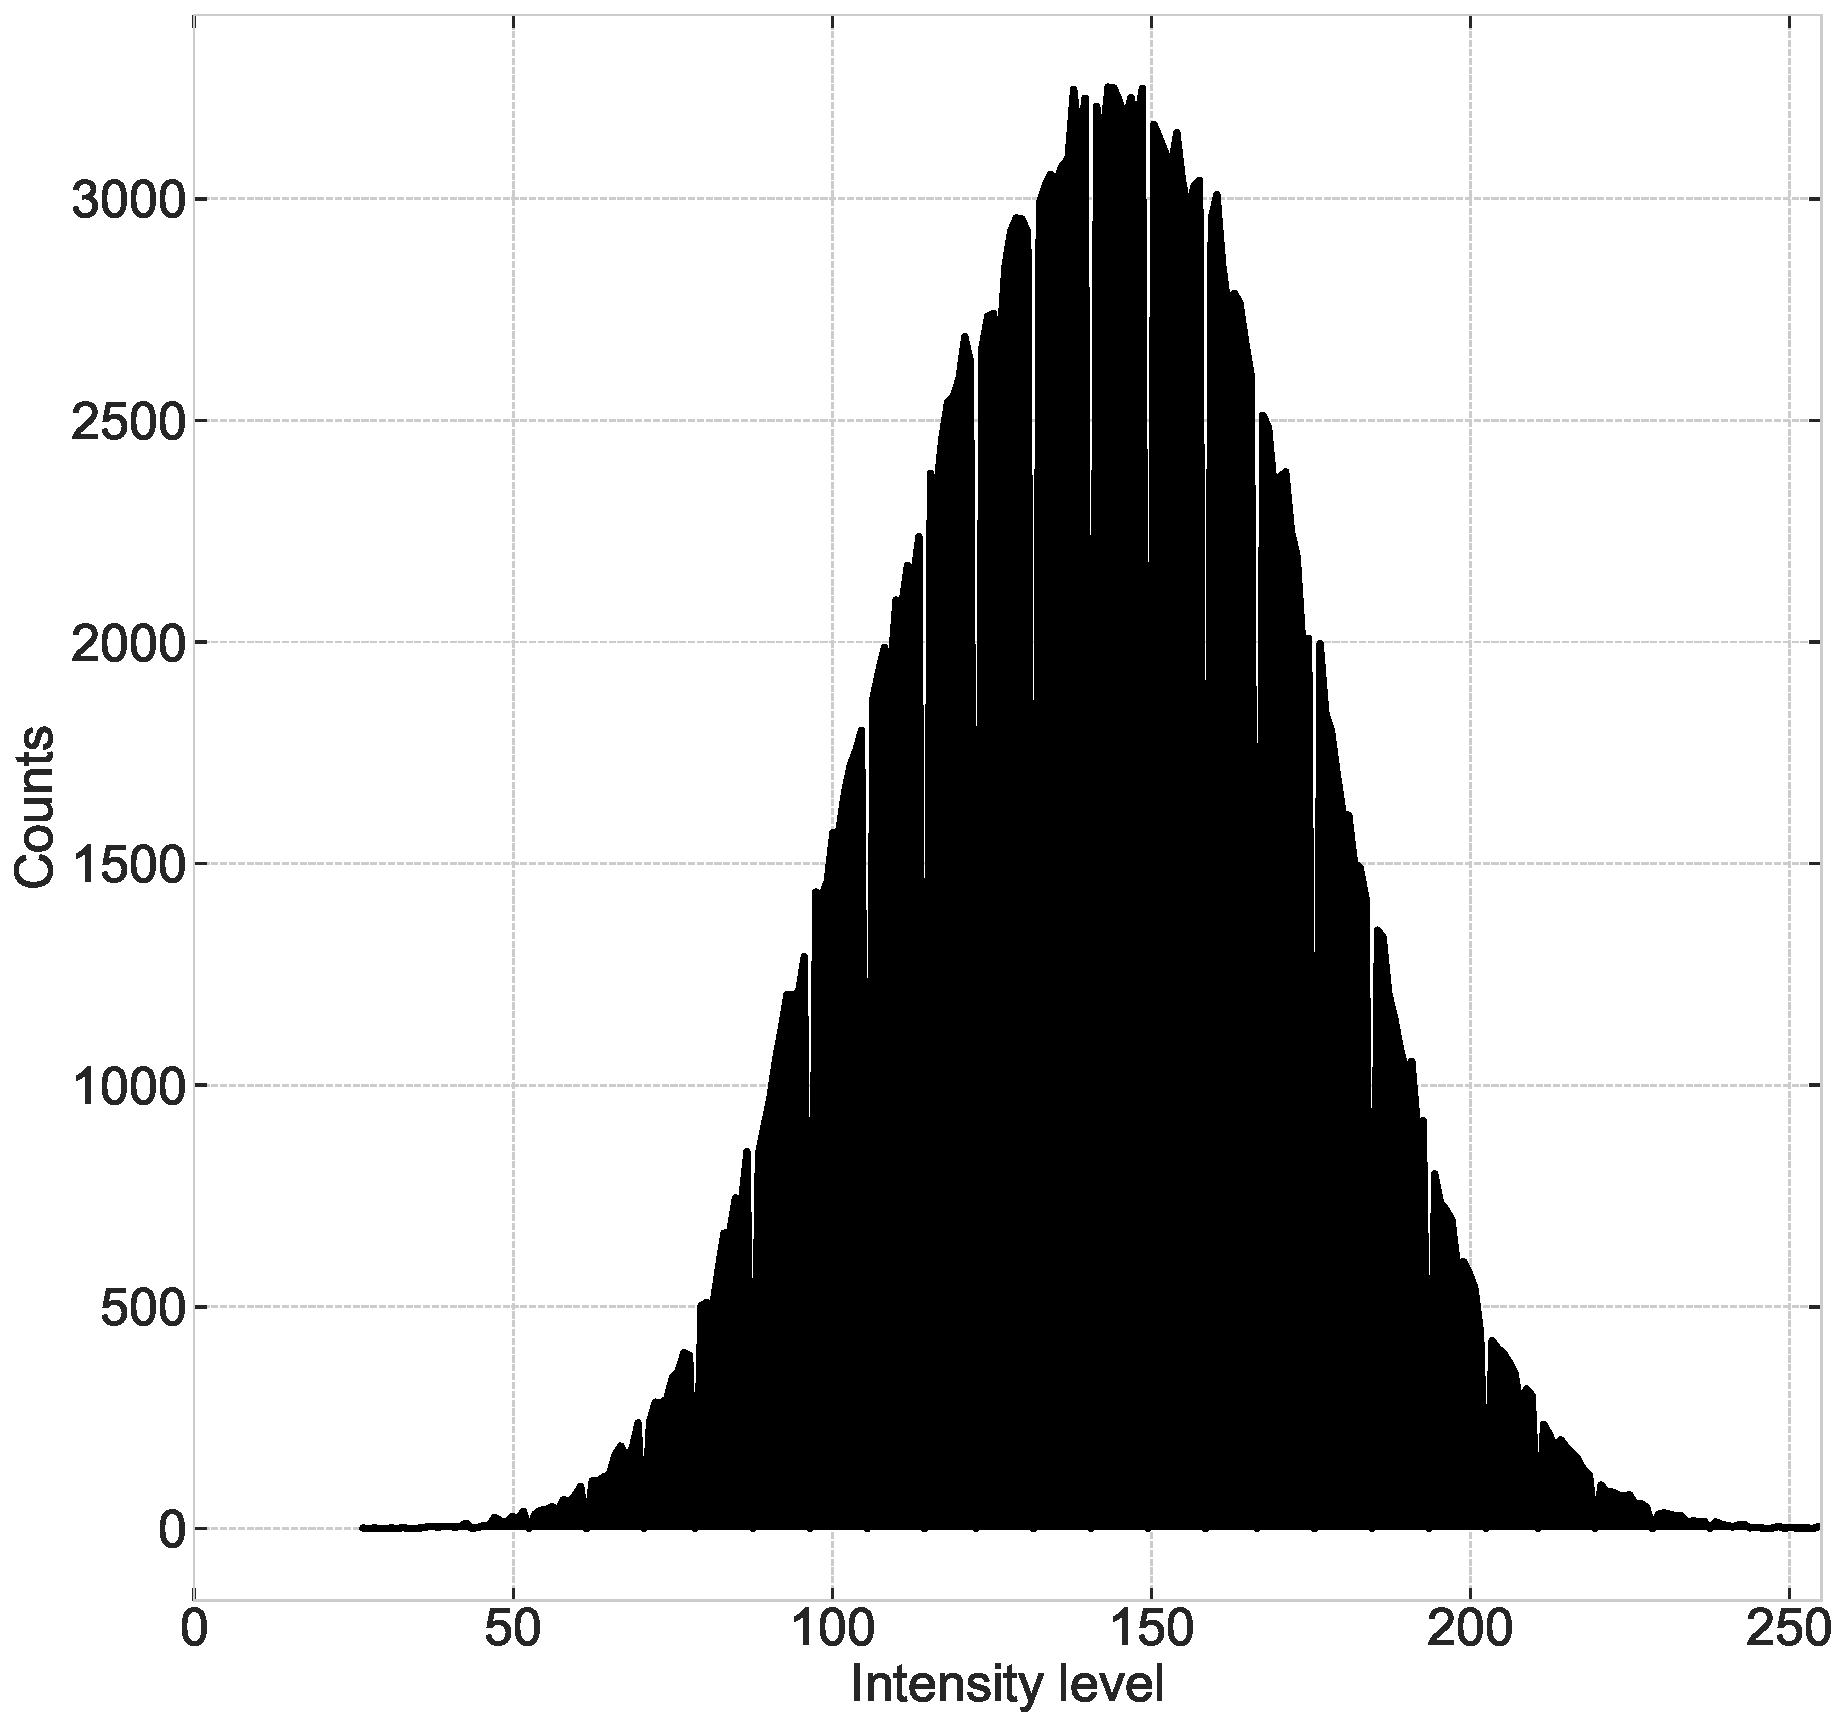
\includegraphics[width=0.8\textwidth]{{img_src/008_a_hist}.pdf}
    \captionof{figure}{Histogram of the image of the microchip with 700x magnitude by detecting secondary electrons.} \label{fig:14}
\end{center}
\vspace*{\fill}
\newpage
\topskip0pt
\vspace*{\fill}
\begin{center}
    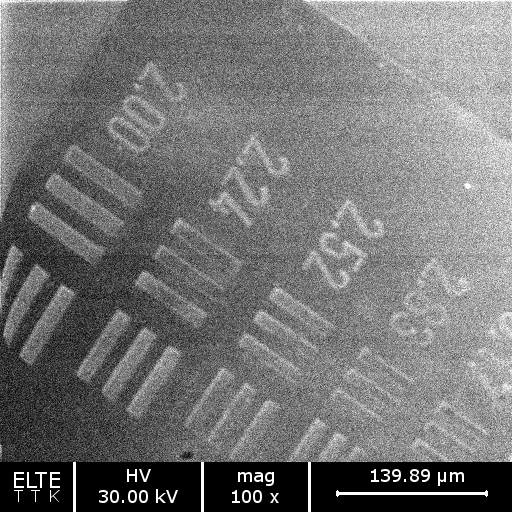
\includegraphics[width=0.8\textwidth]{{img_src/009_a}.png}
    \captionof{figure}{Surface of a microchip with 100x magnitude by detecting secondary electrons.} \label{fig:15}
\end{center}
\begin{center}
    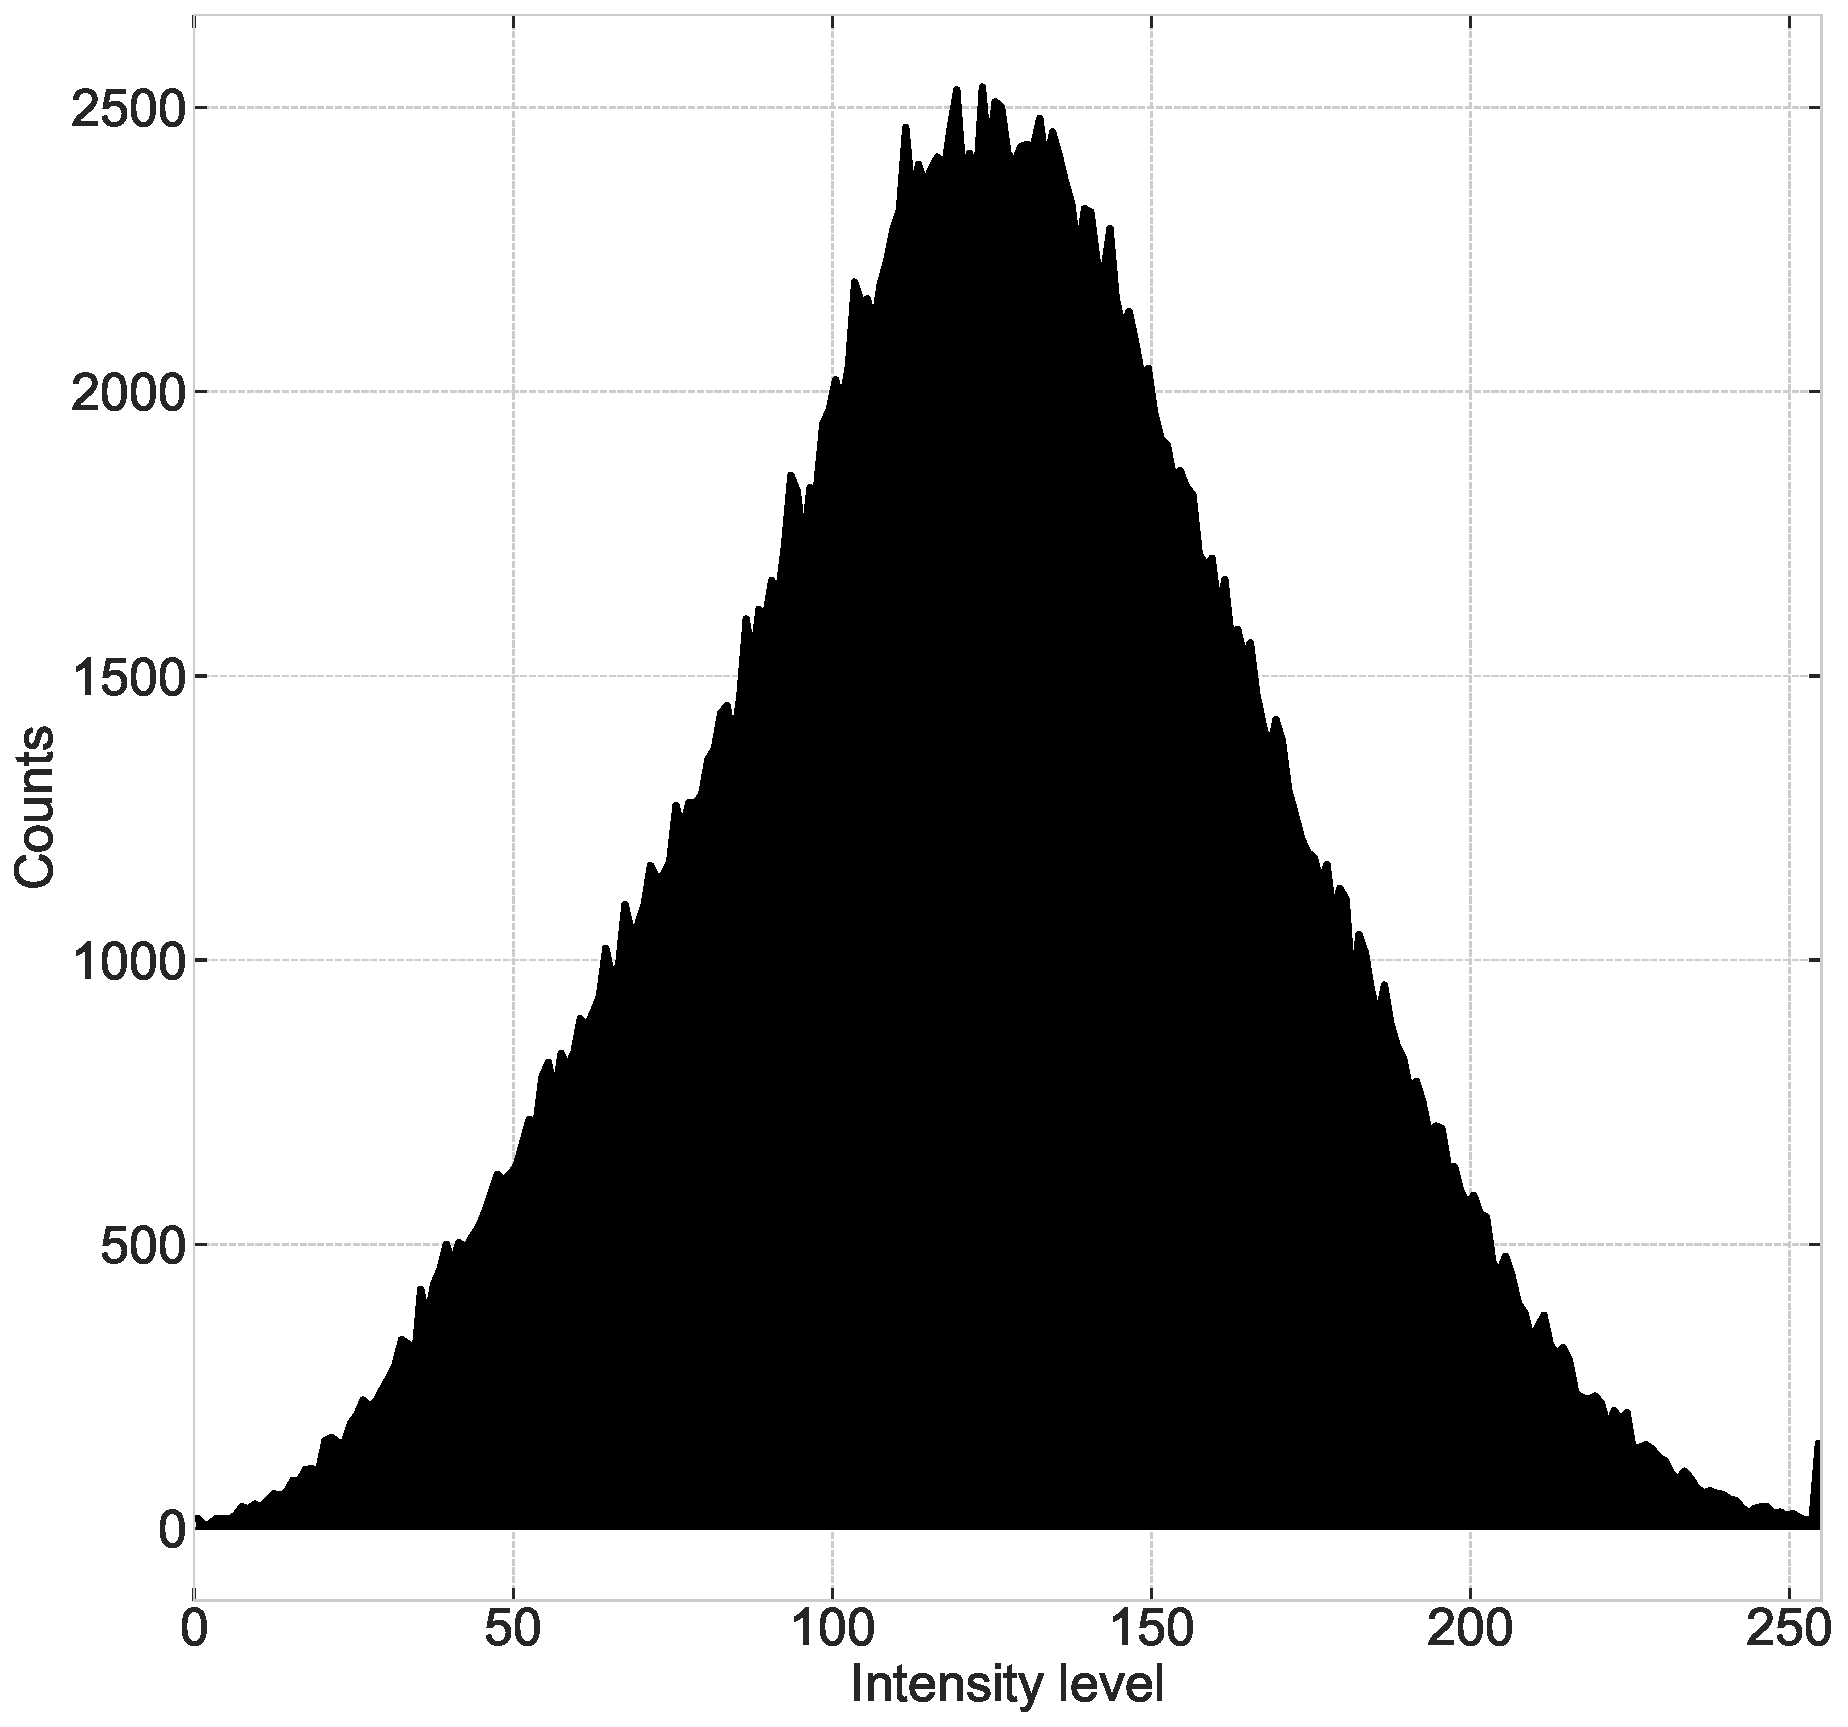
\includegraphics[width=0.8\textwidth]{{img_src/009_a_hist}.pdf}
    \captionof{figure}{Histogram of the image of the microchip hair with 100x magnitude by detecting secondary electrons.} \label{fig:16}
\end{center}
\vspace*{\fill}
\newpage
\topskip0pt
\vspace*{\fill}
\begin{center}
    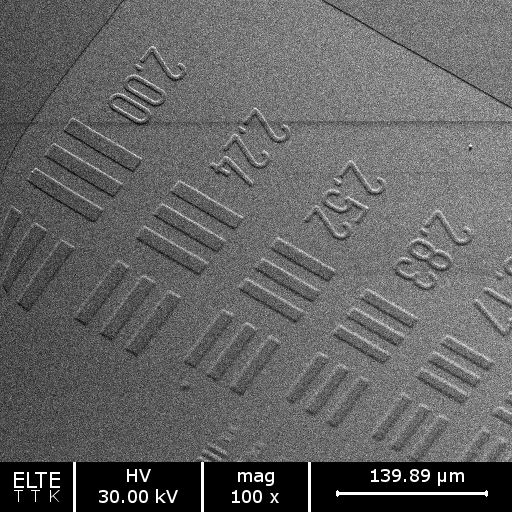
\includegraphics[width=0.8\textwidth]{{img_src/010_a}.png}
    \captionof{figure}{Surface of a microchip with 100x magnitude by detecting backscattered electrons.} \label{fig:17}
\end{center}
\begin{center}
    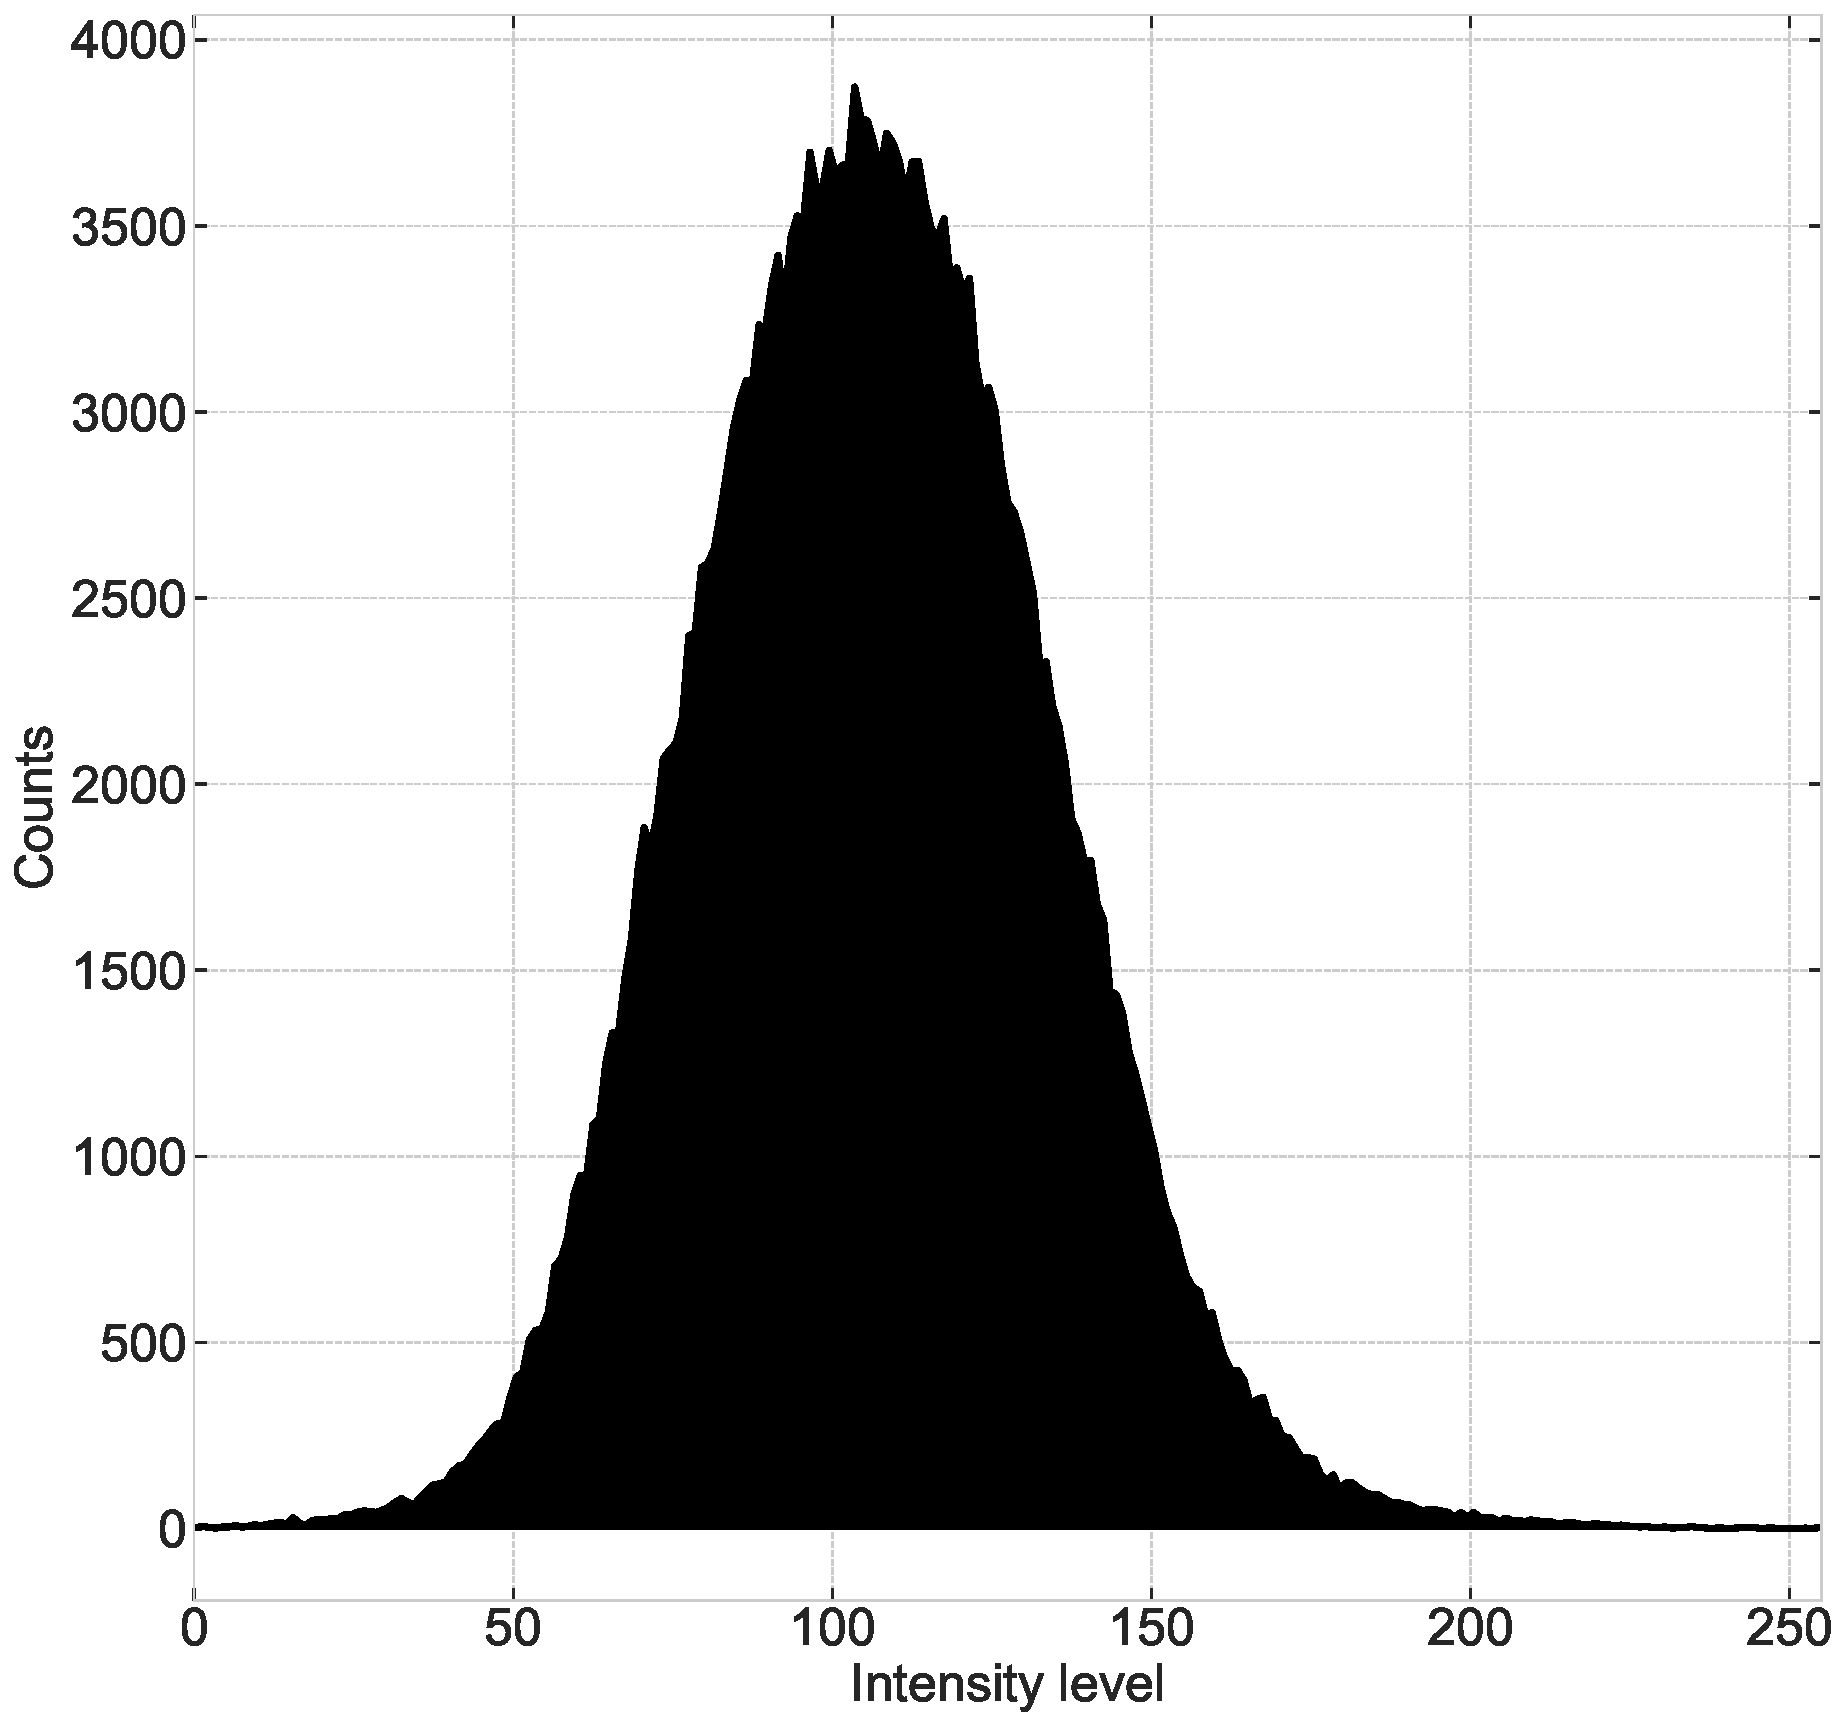
\includegraphics[width=0.8\textwidth]{{img_src/010_a_hist}.pdf}
    \captionof{figure}{Histogram of the image of the microchip with 100x magnitude by detecting backscattered electrons.} \label{fig:18}
\end{center}
\vspace*{\fill}
\newpage